\documentclass[tikz,border=8pt]{standalone}
\usetikzlibrary{arrows.meta,positioning}

\begin{document}
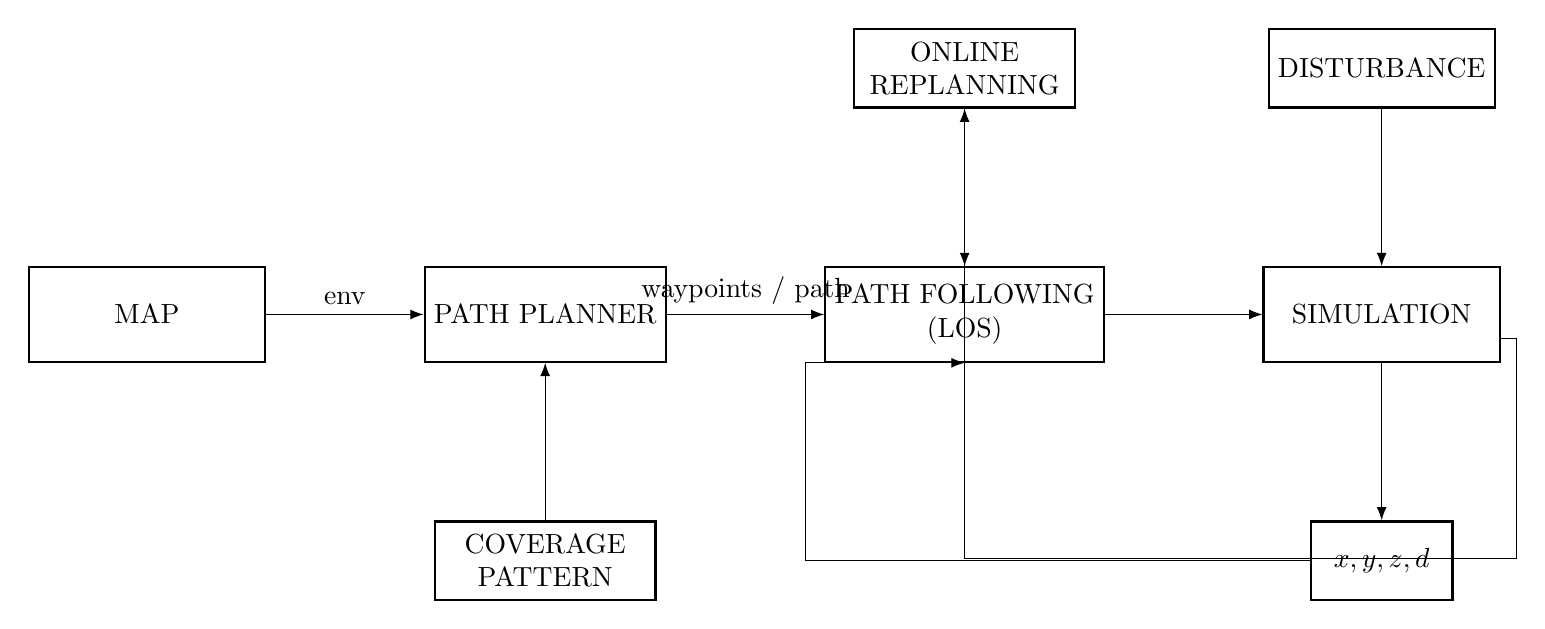
\begin{tikzpicture}[
  block/.style={draw, thick, rectangle, minimum width=30mm, minimum height=12mm, align=center},
  smallblock/.style={draw, thick, rectangle, minimum width=28mm, minimum height=10mm, align=center},
  io/.style={draw, thick, rectangle, minimum width=18mm, minimum height=10mm, align=center},
  >=Latex, node distance=20mm
]

% Nodes left to right
\node[block] (map) {MAP};
\node[block, right=of map] (planner) {PATH PLANNER};
\node[block, right=of planner] (follow) {PATH FOLLOWING\\(LOS)};
\node[block, right=of follow] (sim) {SIMULATION};

% Extra blocks
\node[smallblock, above=of follow] (replan) {ONLINE\\REPLANNING};
\node[smallblock, above=of sim] (dist) {DISTURBANCE};
\node[smallblock, below=of planner] (cov) {COVERAGE\\PATTERN};

% Outputs
\node[io, below=of sim] (out) {$x,y,z,d$};

% Connections
\draw[->] (map) -- node[above]{env} (planner);
\draw[->] (cov) -- (planner);
\draw[->] (planner) -- node[above]{waypoints / path} (follow);
\draw[->] (follow) -- (sim);
\draw[->] (dist) -- (sim);

\draw[->] (sim) -- (out);
\draw[->] (out.west) -- ++(-6.4,0) |- (follow.south);

% Feedback to replanner
\draw[->] (sim.east) ++(0,-0.3) -| ++(0.2,-2.8) -| (replan.south);
\draw[->] (replan.south) -- ++(0,-0.6) -| (follow.north);

\end{tikzpicture}
\end{document}
